\chapter{Probabilidad}

\index{probabilidad}

Una \key{probabilidad} es un número real entre $0$ y $1$
que indica qué tan probable es un evento.
Si un evento está seguro de ocurrir,
su probabilidad es 1,
y si un evento es imposible,
su probabilidad es 0.
La probabilidad de un evento se denota $P(\cdots)$
donde los tres puntos describen el evento.

Por ejemplo, al tirar un dado,
el resultado es un entero entre $1$ y $6$,
y la probabilidad de cada resultado es $1/6$.
Por ejemplo, podemos calcular las siguientes probabilidades:

\begin{itemize}[noitemsep]
\item $P(\textrm{''el resultado es 4''})=1/6$
\item $P(\textrm{''el resultado no es 6''})=5/6$
\item $P(\textrm{''el resultado es par''})=1/2$
\end{itemize}

\section{Cálculo}

Para calcular la probabilidad de un evento,
podemos usar combinatoria
o simular el proceso que genera el evento.
Como ejemplo, calculemos la probabilidad
de sacar tres cartas con el mismo valor
de una baraja de cartas barajada
(por ejemplo, $\spadesuit 8$, $\clubsuit 8$ y $\diamondsuit 8$).

\subsubsection*{Método 1}

Podemos calcular la probabilidad usando la fórmula

\[\frac{\textrm{número de resultados deseados}}{\textrm{número total de resultados}}.\]

En este problema, los resultados deseados son aquellos
en los que el valor de cada carta es el mismo.
Hay $13 {4 \choose 3}$ resultados de este tipo,
porque hay $13$ posibilidades para el
valor de las cartas y ${4 \choose 3}$ formas de
elegir $3$ palos de $4$ palos posibles.

Hay un total de ${52 \choose 3}$ resultados,
porque elegimos 3 cartas de 52 cartas.
Por lo tanto, la probabilidad del evento es

\[\frac{13 {4 \choose 3}}{{52 \choose 3}} = \frac{1}{425}.\]

\subsubsection*{Método 2}

Otra forma de calcular la probabilidad es
simular el proceso que genera el evento.
En este ejemplo, sacamos tres cartas, por lo que el proceso
consiste en tres pasos.
Requerimos que cada paso del proceso sea exitoso.

Sacar la primera carta ciertamente tiene éxito,
porque no hay restricciones.
El segundo paso tiene éxito con una probabilidad de $3/51$,
porque quedan 51 cartas y 3 de ellas
tienen el mismo valor que la primera carta.
De manera similar, el tercer paso tiene éxito con una probabilidad de $2/50$.

La probabilidad de que todo el proceso tenga éxito es

\[1 \cdot \frac{3}{51} \cdot \frac{2}{50} = \frac{1}{425}.\]

\section{Eventos}

Un evento en teoría de la probabilidad se puede representar como un conjunto
\[A \subset X,\]
donde $X$ contiene todos los resultados posibles
y $A$ es un subconjunto de resultados.
Por ejemplo, al sacar un dado, los resultados son
\[X = \{1,2,3,4,5,6\}.\]
Ahora, por ejemplo, el evento ''el resultado es par''
corresponde al conjunto
\[A = \{2,4,6\}.\]

A cada resultado $x$ se le asigna una probabilidad $p(x)$.
Luego, la probabilidad $P(A)$ de un evento
$A$ se puede calcular como una suma
de probabilidades de resultados usando la fórmula
\[P(A) = \sum_{x \in A} p(x).\]
Por ejemplo, al tirar un dado,
$p(x)=1/6$ para cada resultado $x$,
por lo que la probabilidad del evento
''el resultado es par'' es
\[p(2)+p(4)+p(6)=1/2.\]

La probabilidad total de los resultados en $X$ debe
ser 1, es decir, $P(X)=1$.

Dado que los eventos en teoría de la probabilidad son conjuntos,
podemos manipularlos usando operaciones estándar de conjuntos:

\begin{itemize}
\item El \key{complemento} $\bar A$ significa
''$A$ no ocurre''.
Por ejemplo, al tirar un dado, 
el complemento de $A=\{2,4,6\}$ es
$\bar A = \{1,3,5\}$.
\item La \key{unión} $A \cup B$ significa
''$A$ o $B$ ocurren''.
Por ejemplo, la unión de
$A=\{2,5\}$
y $B=\{4,5,6\}$ es
$A \cup B = \{2,4,5,6\}$.
\item La \key{intersección} $A \cap B$ significa
''$A$ y $B$ ocurren''.
Por ejemplo, la intersección de
$A=\{2,5\}$ y $B=\{4,5,6\}$ es
$A \cap B = \{5\}$.
\end{itemize}

\subsubsection{Complemento}

La probabilidad del complemento
$\bar A$ se calcula usando la fórmula
\[P(\bar A)=1-P(A).\]

A veces, podemos resolver un problema fácilmente
usando complementos resolviendo el problema opuesto.
Por ejemplo, la probabilidad de obtener
al menos un seis al tirar un dado diez veces es
\[1-(5/6)^{10}.\]

Aquí $5/6$ es la probabilidad de que el resultado
de un solo tiro no sea seis, y
$(5/6)^{10}$ es la probabilidad de que ninguno de
los diez tiros sea un seis.
El complemento de esto es la respuesta al problema.

\subsubsection{Unión}

La probabilidad de la unión $A \cup B$
se calcula usando la fórmula
\[P(A \cup B)=P(A)+P(B)-P(A \cap B).\]
Por ejemplo, al tirar un dado,
la unión de los eventos
\[A=\textrm{''el resultado es par''}\]
y
\[B=\textrm{''el resultado es menor que 4''}\]
es
\[A \cup B=\textrm{''el resultado es par o menor que 4''},\]
y su probabilidad es
\[P(A \cup B) = P(A)+P(B)-P(A \cap B)=1/2+1/2-1/6=5/6.\]

Si los eventos $A$ y $B$ son \key{disjuntos}, es decir,
$A \cap B$ está vacío,
la probabilidad del evento $A \cup B$ es simplemente

\[P(A \cup B)=P(A)+P(B).\]

\subsubsection{Probabilidad condicional}

\index{probabilidad condicional}

La \key{probabilidad condicional}
\[P(A | B) = \frac{P(A \cap B)}{P(B)}\]
es la probabilidad de $A$
asumiendo que $B$ sucede.
Por lo tanto, al calcular la
probabilidad de $A$, solo consideramos los resultados
que también pertenecen a $B$.

Usando los conjuntos previos,
\[P(A | B)= 1/3,\]
porque los resultados de $B$ son
$\{1,2,3\}$, y uno de ellos es par.
Esta es la probabilidad de un resultado par
si sabemos que el resultado está entre $1 \ldots 3$.

\subsubsection{Intersección}

\index{independencia}

Usando la probabilidad condicional,
la probabilidad de la intersección
$A \cap B$ se puede calcular usando la fórmula
\[P(A \cap B)=P(A)P(B|A).\]
Los eventos $A$ y $B$ son \key{independientes} si
\[P(A|B)=P(A) \hspace{10px}\textrm{y}\hspace{10px} P(B|A)=P(B),\]
lo que significa que el hecho de que $B$ suceda no
cambia la probabilidad de $A$, y viceversa.
En este caso, la probabilidad de la intersección es
\[P(A \cap B)=P(A)P(B).\]
Por ejemplo, al sacar una carta de una baraja, los eventos
\[A = \textrm{''el palo es trébol''}\]
y
\[B = \textrm{''el valor es cuatro''}\]
son independientes. Por lo tanto, el evento
\[A \cap B = \textrm{''la carta es el cuatro de tréboles''}\]
sucede con probabilidad
\[P(A \cap B)=P(A)P(B)=1/4 \cdot 1/13 = 1/52.\]

\section{Variables aleatorias}

\index{variable aleatoria}

Una \key{variable aleatoria} es un valor que se genera
por un proceso aleatorio.
Por ejemplo, al lanzar dos dados,
una posible variable aleatoria es
\[X=\textrm{''la suma de los resultados''}.\]
Por ejemplo, si los resultados son $[4,6]$
(lo que significa que primero tiramos un cuatro y luego un seis),
entonces el valor de $X$ es 10.

Denotamos $P(X=x)$ la probabilidad de que
el valor de una variable aleatoria $X$ es $x$.
Por ejemplo, al lanzar dos dados,
$P(X=10)=3/36$,
porque el número total de resultados es 36
y hay tres formas posibles de obtener
la suma 10: $[4,6]$, $[5,5]$ y $[6,4]$.

\subsubsection{Valor esperado}

\index{valor esperado}

El \key{valor esperado} $E[X]$ indica el
valor promedio de una variable aleatoria $X$.
El valor esperado se puede calcular como la suma
\[\sum_x P(X=x)x,\]
donde $x$ recorre todos los valores posibles de $X$.

Por ejemplo, al lanzar un dado,
el resultado esperado es
\[1/6 \cdot 1 + 1/6 \cdot 2 + 1/6 \cdot 3 + 1/6 \cdot 4 + 1/6 \cdot 5 + 1/6 \cdot 6 = 7/2.\]

Una propiedad útil de los valores esperados es \key{linealidad}.
Significa que la suma
$E[X_1+X_2+\cdots+X_n]$
siempre es igual a la suma
$E[X_1]+E[X_2]+\cdots+E[X_n]$.
Esta fórmula se cumple incluso si las variables aleatorias
dependen unas de otras.

Por ejemplo, al lanzar dos dados,
la suma esperada es
\[E[X_1+X_2]=E[X_1]+E[X_2]=7/2+7/2=7.\]

Consideremos ahora un problema donde
$n$ bolas se colocan aleatoriamente en $n$ cajas,
y nuestra tarea es calcular el número esperado
de cajas vacías.
Cada bola tiene una probabilidad igual de
ser colocada en cualquiera de las cajas.
Por ejemplo, si $n=2$, las posibilidades
son las siguientes:
\begin{center}
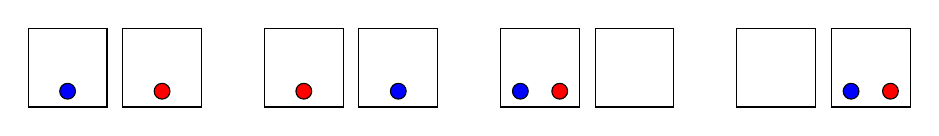
\begin{tikzpicture}
\draw (0,0) rectangle (1,1);
\draw (1.2,0) rectangle (2.2,1);
\draw (3,0) rectangle (4,1);
\draw (4.2,0) rectangle (5.2,1);
\draw (6,0) rectangle (7,1);
\draw (7.2,0) rectangle (8.2,1);
\draw (9,0) rectangle (10,1);
\draw (10.2,0) rectangle (11.2,1);

\draw[fill=blue] (0.5,0.2) circle (0.1);
\draw[fill=red] (1.7,0.2) circle (0.1);
\draw[fill=red] (3.5,0.2) circle (0.1);
\draw[fill=blue] (4.7,0.2) circle (0.1);
\draw[fill=blue] (6.25,0.2) circle (0.1);
\draw[fill=red] (6.75,0.2) circle (0.1);
\draw[fill=blue] (10.45,0.2) circle (0.1);
\draw[fill=red] (10.95,0.2) circle (0.1);
\end{tikzpicture}
\end{center}
En este caso, el número esperado de
cajas vacías es
\[\frac{0+0+1+1}{4} = \frac{1}{2}.\]
En el caso general, la probabilidad de que a
una sola caja esté vacía es
\[\Big(\frac{n-1}{n}\Big)^n,\]
porque ninguna bola debe ser colocada en ella.
Por lo tanto, usando la linealidad, el número esperado de
cajas vacías es
\[n \cdot \Big(\frac{n-1}{n}\Big)^n.\]

\subsubsection{Distribuciones}

\index{distribución}

La \key{distribución} de una variable aleatoria $X$
muestra la probabilidad de cada valor que
$X$ puede tener.
La distribución consiste en valores $P(X=x)$.
Por ejemplo, al lanzar dos dados,
la distribución para su suma es:
\begin{center}
\small {
\begin{tabular}{r|rrrrrrrrrrrrr}
$x$ & 2 & 3 & 4 & 5 & 6 & 7 & 8 & 9 & 10 & 11 & 12 \\
$P(X=x)$ & $1/36$ & $2/36$ & $3/36$ & $4/36$ & $5/36$ & $6/36$ & $5/36$ & $4/36$ & $3/36$ & $2/36$ & $1/36$ \\
\end{tabular}
}
\end{center}

\index{distribución uniforme}
En una \key{distribución uniforme},
la variable aleatoria $X$ tiene $n$ posibles
valores $a,a+1,\ldots,b$ y la probabilidad de cada valor es $1/n$.
Por ejemplo, al lanzar un dado,
$a=1$, $b=6$ y $P(X=x)=1/6$ para cada valor $x$.

El valor esperado de $X$ en una distribución uniforme es
\[E[X] = \frac{a+b}{2}.\]
\index{binomial distribution}
En una \key{distribución binomial}, se realizan $n$ intentos
y la probabilidad de que un solo intento tenga éxito
es $p$.
La variable aleatoria $X$ cuenta el número de
intentos exitosos,
y la probabilidad de un valor $x$ es
\[P(X=x)=p^x (1-p)^{n-x} {n \choose x},\]
donde $p^x$ y $(1-p)^{n-x}$ corresponden a
intentos exitosos y fallidos,
y ${n \choose x}$ es el número de formas
en que podemos elegir el orden de los intentos.

Por ejemplo, al lanzar un dado diez veces,
la probabilidad de obtener un seis exactamente
tres veces es $(1/6)^3 (5/6)^7 {10 \choose 3}$.

El valor esperado de $X$ en una distribución binomial es
\[E[X] = pn.\]

\index{geometric distribution}
En una \key{distribución geométrica},
la probabilidad de que un intento tenga éxito es $p$,
y continuamos hasta que ocurre el primer éxito.
La variable aleatoria $X$ cuenta el número
de intentos necesarios, y la probabilidad de
un valor $x$ es
\[P(X=x)=(1-p)^{x-1} p,\]
donde $(1-p)^{x-1}$ corresponde a los intentos fallidos
y $p$ corresponde al primer intento exitoso.

Por ejemplo, si lanzamos un dado hasta que obtengamos un seis,
la probabilidad de que el número de lanzamientos
sea exactamente 4 es $(5/6)^3 1/6$.

El valor esperado de $X$ en una distribución geométrica es
\[E[X]=\frac{1}{p}.\]

\section{Cadenas de Markov}

\index{Markov chain}

Una \key{cadena de Markov}
% \footnote{A. A. Markov (1856--1922)
% fue un matemático ruso.}
es un proceso aleatorio
que consiste en estados y transiciones entre ellos.
Para cada estado, conocemos las probabilidades
de pasar a otros estados.
Una cadena de Markov puede representarse como un gráfico
cuyos nodos son estados y los bordes son transiciones.

Como ejemplo, considere un problema
donde estamos en el piso 1 de un edificio de $n$ pisos.
En cada paso, caminamos aleatoriamente un piso
hacia arriba o un piso hacia abajo, excepto que siempre
caminamos un piso hacia arriba desde el piso 1 y un piso hacia abajo
desde el piso $n$.
¿Cuál es la probabilidad de estar en el piso $m$
después de $k$ pasos?

En este problema, cada piso del edificio
corresponde a un estado en una cadena de Markov.
Por ejemplo, si $n=5$, el gráfico es el siguiente:

\begin{center}
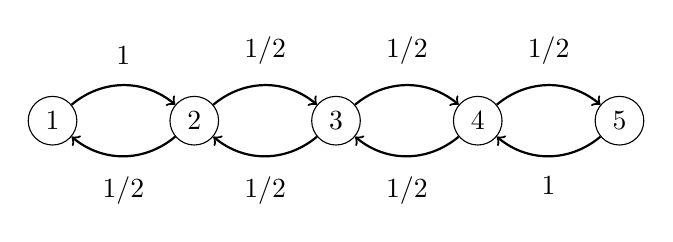
\begin{tikzpicture}[scale=0.9]
\node[draw, circle] (1) at (0,0) {$1$};
\node[draw, circle] (2) at (2,0) {$2$};
\node[draw, circle] (3) at (4,0) {$3$};
\node[draw, circle] (4) at (6,0) {$4$};
\node[draw, circle] (5) at (8,0) {$5$};

\path[draw,thick,->] (1) edge [bend left=40] node[font=\small,label=$1$] {} (2);
\path[draw,thick,->] (2) edge [bend left=40] node[font=\small,label=$1/2$] {} (3);
\path[draw,thick,->] (3) edge [bend left=40] node[font=\small,label=$1/2$] {} (4);
\path[draw,thick,->] (4) edge [bend left=40] node[font=\small,label=$1/2$] {} (5);

\path[draw,thick,->] (5) edge [bend left=40] node[font=\small,label=below:$1$] {} (4);
\path[draw,thick,->] (4) edge [bend left=40] node[font=\small,label=below:$1/2$] {} (3);
\path[draw,thick,->] (3) edge [bend left=40] node[font=\small,label=below:$1/2$] {} (2);
\path[draw,thick,->] (2) edge [bend left=40] node[font=\small,label=below:$1/2$] {} (1);

%\path[draw,thick,->] (1) edge [bend left=40] node[font=\small,label=below:$1$] {} (2);
\end{tikzpicture}
\end{center}

La distribución de probabilidad
de una cadena de Markov es un vector
$[p_1,p_2,\ldots,p_n]$, donde $p_k$ es la
probabilidad de que el estado actual sea $k$.
La fórmula $p_1+p_2+\cdots+p_n=1$ siempre se cumple.

En el escenario anterior, la distribución inicial es
$[1,0,0,0,0]$, porque siempre comenzamos en el piso 1.
La siguiente distribución es $[0,1,0,0,0]$,
porque solo podemos movernos del piso 1 al piso 2.
Después de esto, podemos movernos un piso hacia arriba
o un piso hacia abajo, por lo que la siguiente distribución es
$[1/2,0,1/2,0,0]$, y así sucesivamente.

Una forma eficiente de simular la caminata en
una cadena de Markov es usar la programación dinámica.
La idea es mantener la distribución de probabilidad,
y en cada paso recorrer todas las posibilidades
de cómo podemos movernos.
Usando este método, podemos simular
una caminata de $m$ pasos en $O(n^2 m)$ tiempo.

Las transiciones de una cadena de Markov también pueden
representarse como una matriz que actualiza la
distribución de probabilidad.
En el escenario anterior, la matriz es

\[ 
 \begin{bmatrix}
  0 & 1/2 & 0 & 0 & 0 \\
  1 & 0 & 1/2 & 0 & 0 \\
  0 & 1/2 & 0 & 1/2 & 0 \\
  0 & 0 & 1/2 & 0 & 1 \\
  0 & 0 & 0 & 1/2 & 0 \\
 \end{bmatrix}.
\]

Cuando multiplicamos una distribución de probabilidad por esta matriz,
obtenemos la nueva distribución después de movernos un paso.
Por ejemplo, podemos movernos desde la distribución
$[1,0,0,0,0]$ a la distribución
$[0,1,0,0,0]$ de la siguiente manera:

\[ 
 \begin{bmatrix}
  0 & 1/2 & 0 & 0 & 0 \\
  1 & 0 & 1/2 & 0 & 0 \\
  0 & 1/2 & 0 & 1/2 & 0 \\
  0 & 0 & 1/2 & 0 & 1 \\
  0 & 0 & 0 & 1/2 & 0 \\
 \end{bmatrix}
 \begin{bmatrix}
  1 \\
  0 \\
  0 \\
  0 \\
  0 \\
 \end{bmatrix}
=
 \begin{bmatrix}
  0 \\
  1 \\
  0 \\
  0 \\
  0 \\
 \end{bmatrix}.
\]

Calculando potencias de matrices de manera eficiente,
podemos calcular la distribución después de $m$ pasos
en $O(n^3 \log m)$ tiempo.

\section{Algoritmos aleatorios}

\index{randomized algorithm}


A veces podemos usar la aleatoriedad para resolver un problema,
incluso si el problema no está relacionado con las probabilidades.
Un \key{algoritmo aleatorio} es un algoritmo que
se basa en la aleatoriedad.

\index{Algoritmo de Monte Carlo}

Un \key{algoritmo de Monte Carlo} es un algoritmo aleatorio
que a veces puede dar una respuesta incorrecta.
Para que tal algoritmo sea útil,
la probabilidad de una respuesta incorrecta debe ser pequeña.

\index{Algoritmo de Las Vegas}

Un \key{algoritmo de Las Vegas} es un algoritmo aleatorio
que siempre da la respuesta correcta,
pero su tiempo de ejecución varía aleatoriamente.
El objetivo es diseñar un algoritmo que sea
eficiente con alta probabilidad.

A continuación, veremos tres problemas de ejemplo que
se pueden resolver utilizando la aleatoriedad.

\subsubsection{Estadística de orden}

\index{estadística de orden}

La $k$-ésima \key{estadística de orden} de una matriz
es el elemento en la posición $k$ después de ordenar
la matriz en orden creciente.
Es fácil calcular cualquier estadística de orden
en tiempo $O(n \log n)$ primero ordenando la matriz,
pero ¿es realmente necesario ordenar toda la matriz
solo para encontrar un elemento?

Resulta que podemos encontrar estadísticas de orden
usando un algoritmo aleatorio sin ordenar la matriz.
El algoritmo, llamado \key{quickselect}\footnote{En 1961,
C. A. R. Hoare publicó dos algoritmos que
son eficientes en promedio: \index{quicksort} \index{quickselect}
\key{quicksort} \cite{hoa61a} para ordenar matrices y
\key{quickselect} \cite{hoa61b} para encontrar estadísticas de orden.}, es un algoritmo de Las Vegas:
su tiempo de ejecución suele ser $O(n)$
pero $O(n^2)$ en el peor de los casos.

El algoritmo elige un elemento aleatorio $x$
de la matriz, y mueve los elementos más pequeños que $x$
a la parte izquierda de la matriz,
y todos los demás elementos a la parte derecha de la matriz.
Esto lleva $O(n)$ tiempo cuando hay $n$ elementos.
Supongamos que la parte izquierda contiene $a$ elementos
y la parte derecha contiene $b$ elementos.
Si $a=k$, el elemento $x$ es la $k$-ésima estadística de orden.
De lo contrario, si $a>k$, encontramos recursivamente la $k$-ésima orden
estadística para la parte izquierda,
y si $a<k$, encontramos recursivamente la $r$-ésima orden
estadística para la parte derecha donde $r=k-a$.
La búsqueda continúa de manera similar, hasta que el elemento
se ha encontrado.

Cuando cada elemento $x$ se elige aleatoriamente,
el tamaño de la matriz se reduce aproximadamente a la mitad en cada paso,
por lo que la complejidad temporal para
encontrar la $k$-ésima estadística de orden es aproximadamente
\[n+n/2+n/4+n/8+\cdots < 2n = O(n).\]

El peor caso del algoritmo todavía requiere $O(n^2)$ tiempo,
porque es posible que $x$ siempre se elija
de tal manera que sea uno de los elementos más pequeños o más grandes
de la matriz y se necesitan $O(n)$ pasos.
Sin embargo, la probabilidad de esto es tan pequeña
que esto nunca sucede en la práctica.

\subsubsection{Verificación de la multiplicación de matrices}

\index{multiplicación de matrices}

Nuestro siguiente problema es \emph{verificar}
si $AB=C$ se cumple cuando $A$, $B$ y $C$
son matrices de tamaño $n \times n$.
Por supuesto, podemos resolver el problema
calculando el producto $AB$ de nuevo
(en tiempo $O(n^3)$ usando el algoritmo básico),
pero uno podría esperar que la verificación de la
respuesta sería más fácil que calcularla desde cero.

Resulta que podemos resolver el problema
utilizando un algoritmo de Monte Carlo\footnote{R. M. Freivalds publicó
este algoritmo en 1977 \cite{fre77}, y a veces
se llama \index{algoritmo de Freivalds} \key{algoritmo de Freivalds}.} cuyo
la complejidad temporal es solo $O(n^2)$.
La idea es simple: elegimos un vector aleatorio
$X$ de $n$ elementos, y calculamos las matrices
$ABX$ y $CX$. Si $ABX=CX$, informamos que $AB=C$,
y de lo contrario informamos que $AB \neq C$.

La complejidad temporal del algoritmo es
$O(n^2)$, porque podemos calcular las matrices
$ABX$ y $CX$ en tiempo $O(n^2)$.
Podemos calcular la matriz $ABX$ de manera eficiente
utilizando la representación $A(BX)$, por lo que solo dos
multiplicaciones de $n \times n$ y $n \times 1$
matrices de tamaño son necesarios.

El inconveniente del algoritmo es
que existe una pequeña posibilidad de que el algoritmo
cometa un error cuando informa que $AB=C$.
Por ejemplo, 
\[
 \begin{bmatrix}
  6 & 8 \\
  1 & 3 \\
 \end{bmatrix}
\neq
 \begin{bmatrix}
  8 & 7 \\
  3 & 2 \\
 \end{bmatrix},
\]
pero
\[
 \begin{bmatrix}
  6 & 8 \\
  1 & 3 \\
 \end{bmatrix}
 \begin{bmatrix}
  3 \\
  6 \\
 \end{bmatrix}
=
 \begin{bmatrix}
  8 & 7 \\
  3 & 2 \\
 \end{bmatrix}
 \begin{bmatrix}
  3 \\
  6 \\
 \end{bmatrix}.
\]
Sin embargo, en la práctica, la probabilidad de que el
algoritmo cometa un error es pequeña,
y podemos disminuir la probabilidad mediante
la verificación del resultado usando múltiples vectores aleatorios $X$
antes de informar que $AB=C$.

\subsubsection{Coloración de grafos}

\index{coloración}
Dado un grafo que contiene $n$ nodos y $m$ aristas,
nuestra tarea es encontrar una forma de colorear los nodos
del grafo usando dos colores de modo que
para al menos $m/2$ aristas, los puntos finales 
tengan colores diferentes.
Por ejemplo, en el grafo
\begin{center}
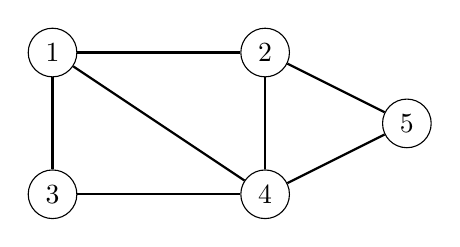
\begin{tikzpicture}[scale=0.9]
\node[draw, circle] (1) at (1,3) {$1$};
\node[draw, circle] (2) at (4,3) {$2$};
\node[draw, circle] (3) at (1,1) {$3$};
\node[draw, circle] (4) at (4,1) {$4$};
\node[draw, circle] (5) at (6,2) {$5$};

\path[draw,thick,-] (1) -- (2);
\path[draw,thick,-] (1) -- (3);
\path[draw,thick,-] (1) -- (4);
\path[draw,thick,-] (3) -- (4);
\path[draw,thick,-] (2) -- (4);
\path[draw,thick,-] (2) -- (5);
\path[draw,thick,-] (4) -- (5);
\end{tikzpicture}
\end{center}
una coloración válida es la siguiente:
\begin{center}
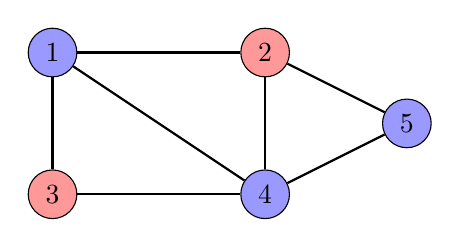
\begin{tikzpicture}[scale=0.9]
\node[draw, circle, fill=blue!40] (1) at (1,3) {$1$};
\node[draw, circle, fill=red!40] (2) at (4,3) {$2$};
\node[draw, circle, fill=red!40] (3) at (1,1) {$3$};
\node[draw, circle, fill=blue!40] (4) at (4,1) {$4$};
\node[draw, circle, fill=blue!40] (5) at (6,2) {$5$};

\path[draw,thick,-] (1) -- (2);
\path[draw,thick,-] (1) -- (3);
\path[draw,thick,-] (1) -- (4);
\path[draw,thick,-] (3) -- (4);
\path[draw,thick,-] (2) -- (4);
\path[draw,thick,-] (2) -- (5);
\path[draw,thick,-] (4) -- (5);
\end{tikzpicture}
\end{center}
El grafo anterior contiene 7 aristas, y para 5 de ellas,
los puntos finales tienen colores diferentes,
por lo que la coloración es válida.

El problema se puede resolver usando un algoritmo de Las Vegas
que genera coloraciones aleatorias hasta que se encuentra una coloración válida.
En una coloración aleatoria, el color de cada nodo es
elegido independientemente de modo que la probabilidad de
ambos colores es $1/2$.

En una coloración aleatoria, la probabilidad de que los puntos finales
de una sola arista tengan colores diferentes es $1/2$.
Por lo tanto, el número esperado de aristas cuyos puntos finales
tienen colores diferentes es $m/2$.
Dado que se espera que una coloración aleatoria sea válida,
encontraremos rápidamente una coloración válida en la práctica.
